


% Recent work in ML interpretability seeks to provide explanations for the models behavior by investgating their inner activations. However, previous work presented either analysis of high level behavior lacking a precise description of their implementation inside the model, or thorough investigation of simple low-level linguistic abilities. In this work, we attempt to bridge this gap by presenting evidence for a circuit in GPT-2 small performing a hihg-level natural language task: indirect object identification. It requires composing different level of linguistic processing to identify subjects from different clauses and predict the entity affected by an action. The circuit is composed of 26 attention heads grouped into 6 main classes, which we discovered using a combination of interpretability tools including causal intervention on activations and embedding projection. To evaluate the reliability of our explanation, we propose three quantitative criteria---\emph{faithfulness, completeness, minimality}---as \todo{make these less important} well as a qualitative requirement for \emph{legibility}. Though our quantitative criteria support our understanding of the structure of the circuit, our explanation doesn't resist adversarial robustness tests and there remain gaps in our understanding of the interaction between components. Our work provides evidence that a mechanistic understanding of large ML models is possible, opening opportunities to scale our understanding to both larger models and more complex tasks.



\section{Introduction}
\label{sec:intro}

% --------------------------------------
% Mechanistic Interpretability outline
% --------------------------------------

% \av{Add: why this task , description of the different class of heads,
% Different part of the circuit and what they do (some are weird),
% High level presentation of the 4 criteria}

 Transformer-based language models \citep{Attention,GPT3} have demonstrated an impressive suite of capabilities but largely remain black boxes. Understanding these models is difficult because they employ complex non-linear interactions in densely-connected layers and operate in a high-dimensional space. Despite this, they are already deployed in high-impact settings \citep{zhang2022shifting, caldarini2022literature},  underscoring the urgency of understanding and anticipating possible model behaviors. Some researchers have argued that interpretability is critical for the safe deployment of advanced machine learning systems \citep{Hendrycks2022XRiskAF}.
%Thus, applying interpretability to language models, which are on the path to create significant real-world impact \citep{RisksAndOpps}, is both challenging and important. 
% \citep{hendrycks2021unsolved}
% \citep{molnar2019}

Work in mechanistic interpretability aims to discover, understand, and verify the algorithms that model weights implement by reverse engineering model computation into human-understandable components \citep{AnthropicMechanisticEssay, meng2022locating, geiger2021causal, geva2020transformer}. By understanding underlying mechanisms, we can better predict out-of-distribution behavior \citep{mu2020compositionalExplanations}, identify and fix model errors \citep{hernandez2021natural,vig2020investigating}, and understand emergent behavior \citep{meca_interp_grokking,barak2022hidden,Wei2022EmergentAO}.

In this work, we aim to mechanistically understand how GPT-2 small \citep{GPT2} implements a simple natural language task. We do so by using \emph{circuit analysis} \citep{interp_survey}, identifying an induced subgraph of the model's computational graph that is human-understandable and responsible for completing the task.

%we locate components of the network that produce specific behaviors, and study how they compose to complete the task.

%To do so, we locate human-understandable components of the network whose behavior composes together to complete the task.

%Specifically, we discover \emph{circuits}: induced subgraphs of a model's computational graph that are human-understandable and responsible for a behavior. % Understanding the semantic functions of the circuit is the main goal of our qualitative criteria: \emph{legibility}. 
%We employed a number of techniques, most notably activation patching, knockouts, which we believe are useful, general techniques for circuit discovery.

To discover the circuit, we introduce a systematic approach that iteratively traces important components back from the logits, using a causal intervention that we call ``path patching". We supplement this mainline approach with projections in the embedding space, attention pattern analysis, and activation patching to understand the behavior of each component.

% In these graphs, nodes are components of the model (neurons and attention heads) and edges are the dependencies defined by the model architecture (attention and residual connections). %In this work, we  use a number of techniques for circuit discovery, most notably activation patching, knockouts, and projections\footnote{For a summary of our thoughts on the usefulness of the various techniques we have tried, see Appendix \ref{app:techniques}}.


% In mechanistic interpretability, \textit{circuits} have been found to be a useful abstraction in isolating and reverse engineering how models perform a specific function. In our work, we think of models as computational graphs and circuits as induced subgraphs, where nodes are components of the model (neurons, attention heads, etc.) and edges the dependencies defined by the model architecture. This definition is slightly different from \cite{olah2020zoom}'s definition of circuits, where nodes are \textit{features}, meaningful directions in the latent space of a model, and edges are defined by the model's weights. Our work provides, to the best of our knowledge, the best attempt at fully reverse engineering a natural behavior emerging in a Transformer-based language model.
%the circuit in transformer-based natural language models made of the most human-understandable components. %composed by the most individual understandable modules.%most complex circuit ever found in a transformer-based language model. 
%Our work identifies, to the best of our knowledge, the structure of the largest circuit ever found in a transformer.

 % \ac{feedback we got: we should clarify why we care about `algorithms' and what this even means in the context of ML; I think readers thought we meant either Dijkstra's algorithm, or the backpropagation algorithm...}
 % (\cite{elhage2021mathematical}, \cite{olah2020zoom}) has found the \textit{circuit} abstraction to be fruitful for gaining understanding of higher level components of neural networks once lower level components are understood. 
% Briefly, if \textit{features} are directions in a latent space within a machine learning model, then circuits are sets of features, with connections between such features defined by weights within the model. 
 
% Prior works in mechanistic interpretability (\cite{AnthropicMechanisticEssay}, \cite{elhage2021mathematical}) has proposed the \textit{circuit} abstraction for understanding neural nets, where the information flow in the model can be understood by modelling it with a computational graph. Geiger et al. elaborate on this framework with their \textit{causal abstractions}, weakly mapping the internals of a BERT-based model to a human interpretable causal model that computes a complex natural language inference task, while Goldowsky-Dill et al. explain how a small transformer model computes a simple algorithmic task with stronger identification \todo{cite nix} \av{How to cite Nix?}. 

% Full understanding of large language model capabilities is currently intractable given the diversity of behaviors they exhibit \citep{GPT3}.

%Pre-trained language models use a vocabulary of tens of thousands of tokens to predict all commonly occurring strings of text that occur in natural language. 
%To make our investigation simpler, 
We focus on understanding a specific natural language task  %in GPT-2 small \citep{GPT2}, 
that we call indirect object identification (IOI). In IOI, sentences such as ``When Mary and John went to the store, John gave a drink to'' should be completed with ``Mary''. %Another example of IOI occurs if the second `John' in the sentence is replaced by `Mary': in this case the correct answer is `John'. 
 We chose this task because it is linguistically meaningful and admits an interpretable algorithm: of the two names in the sentence, predict the name that isn't the subject of the last clause. 
%The crispness of the behavior and GPT-2 small's strong performance on the task gave us hope that the underlying circuit would be interpretable. 

We discover a circuit of 26 attention heads--1.1\% of the total number of (head, token position) pairs--that completes the bulk of this task. 
The circuit uses 7 categories of heads (see Figure~\ref{fig:the_circuit}) to implement the algorithm. Together, these heads route information between different name tokens, to the end position, and finally to the output. 
%3 groups of heads (\emph{Duplicate Token}, \emph{Induction} and \emph{Previous-Token}) move information about the repeated name (John) to the repeated name's token position. The heads at that token position (\emph{Subject-Inhibition}) cause 3 groups of heads at the last token position (\emph{Name-Mover}, \emph{Negative Name-Mover}, \emph{Backup Name-Movers}) to update against the repeated name (John) and copy the non-repeated name (Mary) as the output. 
% an algorithm in three steps: i) Identify all previous names in the sentence (e.g. `John', `John', `Mary'). ii) Remove names that are duplicate (`John') iii) Output the remaining name (`Mary'). 
Our work provides, to the best of our knowledge, the most detailed attempt at reverse-engineering an end-to-end behavior in a transformer-based language model. 

By zooming in on a crisp task in a particular model, we obtained several insights about the challenges of mechanistic interpretability. In particular:

\setdefaultleftmargin{1em}{2.2em}{1.87em}{1.7em}{1em}{1em}
\begin{compactitem}
    \item We identified several instances of heads implementing redundant behavior \citep{michel2019sixteen}. The most surprising were ``Backup Name-Mover Heads'', which copy names to the correct position in the output, but only when regular Name-Mover Heads are ablated. This complicates the search for complete mechanisms, as different model structure is found when some components are ablated.% NOTE ARTHUR DELETED % as single-pass ablations may miss important structure.
    \item We found known structures (specifically induction heads \citep{elhage2021mathematical}) that were used in unexpected ways. Thus mainline functionality of a component does not always give a full picture.
    \item Finally, we identified heads reliably writing in the \emph{opposite} direction of the correct answer.
\end{compactitem}

%each function of the part of the circuit, described in section . 
%The heads fall into 7 major categories: \emph{name-mover}, \emph{subject-inhibition}, \emph{duplicate token}, \emph{negative name-mover}, \emph{backup name-movers}, \emph{induction} and \emph{previous-token} 
% While subsets of as few as 13 of these heads can achieve reasonable performance, we find that all 26 heads are necessary to account for the machinery used by GPT-2 small.
\begin{figure*}
\centering
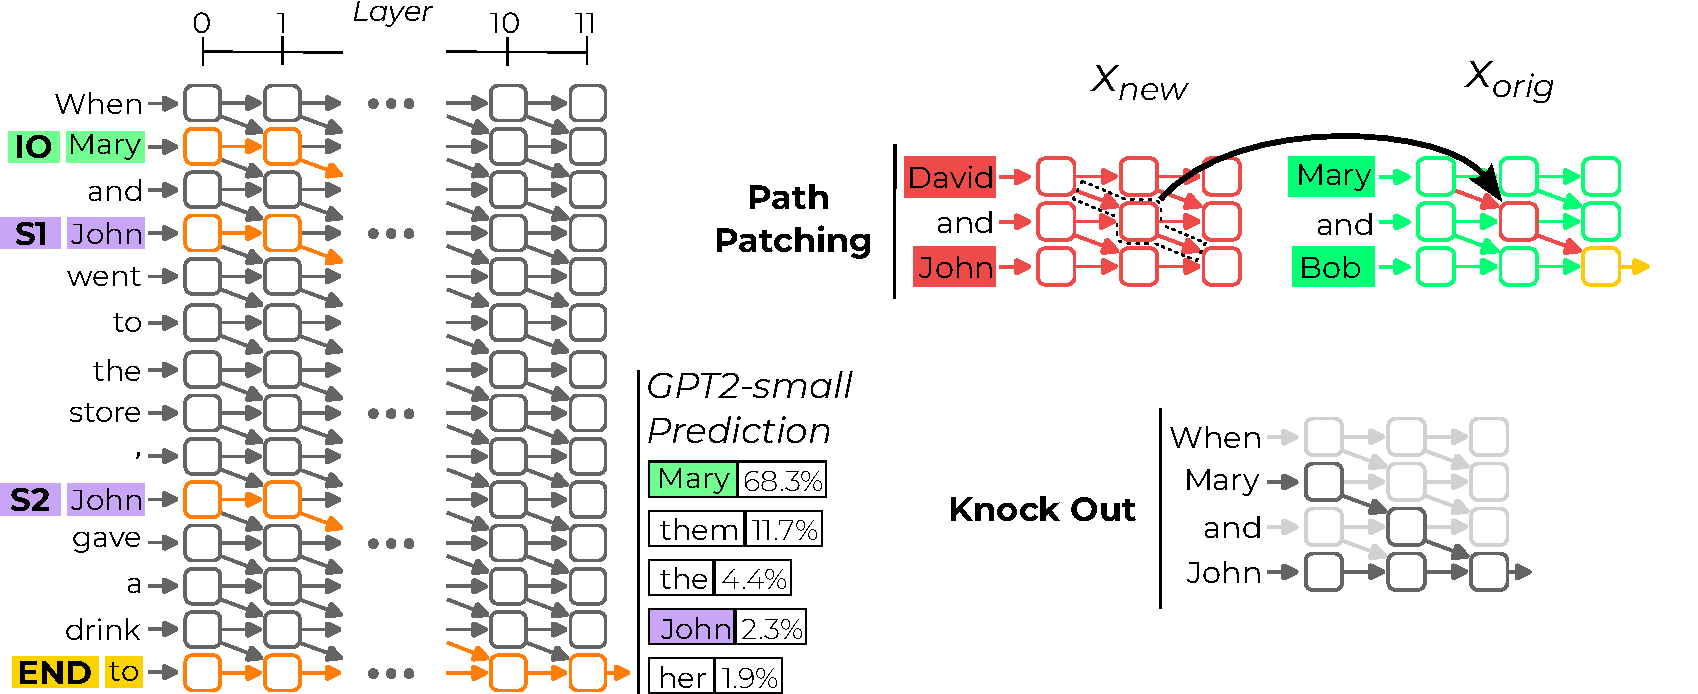
\includegraphics[width=0.8\textwidth]{figs/front_fig_v6.pdf}
\caption{Left: We isolated a \emph{circuit} (in orange) responsible for the flow of information connecting the indirect object ``Mary'' to the next token prediction. The nodes are attention layers and the edges represent the interactions between these layers. Right: We discovered and validated this circuit using causal interventions, including both path patching and knockouts of attention heads.}
\label{fig:directed_graph_figure}
\end{figure*}


Explanations for model behavior can easily be misleading or non-rigorous \citep{attention_not_explanation, interp-illusion-bert}. 
To remedy this problem, we formulate three criteria to help validate our circuit explanations. These criteria are \textbf{faithfulness} (the circuit can perform the task as well as the whole model), \textbf{completeness} (the circuit contains all the nodes used to perform the task), and \textbf{minimality} (the circuit doesn't contain nodes irrelevant to the task). % and \textbf{legibility} (the nodes in the circuit can be mapped to human-understandable concepts).  
Our circuit shows significant improvements compared to a na\"{i}ve (but faithful) circuit, but fails to pass the most challenging tests.

% We empirically evaluate the completeness and minimality criteria using \emph{circuit extraction}: an exhaustive ablation method that isolates a circuit by ablating every node but the circuit. Our circuit passes these tests reasonably, though our understanding is still not complete \ac{I only think we can claim that we pass the tests `better' than other models, not that we objectively pass anything}.
In summary, our main contributions are: (1) We identify a large circuit in GPT-2 small that performs indirect-object identification (Figure \ref{fig:the_circuit} and Section \ref{sec:legibility}); (2) Through example, we identify useful techniques for understanding models, as well as surprising pitfalls;  (3) We present criteria that ensure structural correspondence between the circuit and the model, and check experimentally whether our circuit meets this standard (Section \ref{sec:validation}).
%(3) We check experimentally whether our circuit meets this standard (Sections \ref{sec:legibility} and \ref{sec:validation}).




% --------------------------------------
% the circuit old:
% --------------------------------------
  % old things (4 things!)
    % \item We demonstrate evidence for a sparse circuit in GPT-2 small made of dozens of nodes acting at different point in the sequence to identify indirect objects in natural sentences.
    % \item We present an empirical approach to aim at the identification of complete circuit in GPT models and document use cases of tools.
    % \item We identified classes of heads performing understandable computation that seems to generalize outside the particular task studied.
    % \item We propose theoretical validation criteria for circuit identification in language models, and a practical implementation of them.
% Prior work on such language models (\cite{elhage2021mathematical}) has proposed that the \textit{circuit} abstraction developed from vision models (\cite{olah2020zoom}) is applicable to language models. More generally \textit{causal abstraction}, applied to neural networks in (\cite{geiger2021causal}) aims to understand neural network internals by mapping a human-interpretable causal model to components of a trained neural network. In our work, the causal graph (circuit) has nodes (attention heads, and MLPs in a pretrained transformer) such that it can implement a more complex behaviour than one that the individual nodes can implement alone.

% We group the attention heads in the circuit according to the function they implement. In short, the circuit is composed of:
% \begin{itemize}
%     \item \emph{Name Mover Heads} pay attention to the indirect object that is the only name token that was not marked by \emph{S-Inhibition Heads} and copy its embedding at the final position.

%     \item \emph{Duplicate Token Heads} detect a previous matching token on the subject of the second clause (the second apparition of `John` in the example)
%     \item \emph{Induction Heads} composed with \emph{Previous Token Heads} that were previously described in \cite{AnthropicMechanisticEssay}. Here the induction heads are firing on the subject of the second clause as they detect a pattern of the form \texttt{[A] [B] ... [A]} and are writing \texttt{[B]}. However, the circuit doesn't use the information that is written but the \emph{fact that they write} as an additional duplicate detector.
%     \item \emph{S-Inhibition Heads} are moving the information about the duplicate token to the end position.
%     \item \emph{Negative Heads} behave the same as name movers heads but write in the opposite direction, but with a lesser absolute values compared to name movers heads.
% \end{itemize}
% \av{maybe make this shorter?} 

% Despite the evidence for the structure we identified, we cannot directly trust our understanding as it relies mainly on observation. In particular, we cannot rely on it these methods to test whether our circuit contains all the nodes used to perform IOI.

% Those criteria were designed to strike a balance between the rigor of program proofs, which cannot be applied to the continuous representations and distributed computation of ML models, and a pure empirical approach relying on observation and partial causal interventions. 

% enabling to isolate the effect of a set of nodes while limiting the destructiveness of the intervention on the structure of the natural inner representations. We apply these tests to our proposed circuit and show that it passes reasonably well, however, some of its parts are not yet fully understood and the level of its description could be made more fine-grained.




% --------------------------------------
% IOI (older)
% --------------------------------------

% We claim to have found the outline of a circuit in GPT-2 small (\cite{GPT2}), an auto-regressive language model of 117 million parameters on a natural linguistic task. The task is the next token prediction of an indirect object in a sentence in which the indirect object has already been referred to. For example, in the sentence beginning `When Mary and John went to the store, John gave a drink to' a capable language model should i) predict `Mary' (the indirect object) as a likely next token and ii) not predict `John' (the subject) as the next token. This is because the indirect object of an independent clause can’t be the clause's subject if the verb isn’t reflexive (i.e, `John gave a drink to John' does not make any grammatical sense). \krw{i dont think we should define the task in the intro}

%GPT-2 small empirically consistently meets the requirements i) and ii). Moreover, our work
